\chapter{Introdução}
\label{ch:intro}
\section{Propósito}
    O presente projeto pretende criar um site para gerenciamento de eventos chamado \textit{CriasEvent}, para que os organizadores possam criar e gerenciar eventos, enquanto os participantes possam se inscrever nos mesmos.
\section{Audiência}
    O projeto se destina a organizadores de evento que querem uma plataforma para organizar e disponibilizar seus eventos, tanto presencias como onlines, e para os participantes que desejam se inscrever e participar de eventos, com o diferencial de poderem fazer inscrições para diferentes eventos em uma mesma página.
\section{Uso previsto}
  Espera-se que o site \textit{CriasEvent} seja acessado por usuários cadastrados, que podem ser tanto organizadores quanto participantes. 

  Para participatnes, o site será uma plataforma de inscrição e de consulta, onde o usuário Participante poderá ver quais eventos estão sendo divulgados, e se desejar, se increver nos mesmos, bem como consultar quais eventos já está inscrito. 

  Para organizadores, o site será utilizado para gerenciamento dos eventos, onde os mesmos poderão ser criados, deletados e atualizados pelo organizador, bem como disponibilizados e customizados na página de eventos



\chapter{Descrição Geral}
\label{Descrição Geral}

\section{Classe de Usuários e suas características}
\textit{CriasEvent} tem basicamente três classes de uso:
    \begin{itemize}
        \item \textbf{Organizadores}: Criam e gerenciam seus eventos.
        \item \textbf{Participantes}: Acessam, Buscam e se inscrevem nos eventos disponíveis.
        \item \textbf{Administrador}: Controlam todo o conteúdo do site(Frontend e Backend).
    \end{itemize}

\section{Escopo}
    \textit{CriasEvent} será capaz de:
    \begin{itemize}
      \item Exibição em Interface Web: todos os eventos serão exibidos através de uma página web. 
      \item Gerenciamento de eventos: CRUD dos eventos: Criação, Consulta, Atualização e Remoção de eventos.
      \item Gerenciamento de inscrições: Para participantes haverá Confirmação(testar se o participante pode se inscrever no evento), e para Organizadores haverá acesso a relatórios de inscritos e participantes.
      \item Busca e filtro de eventos: Participantes poderão buscar por eventos baseados em palavras-chave.
      \item Inscrição em eventos.
      \item Acesso às informações detalhadas dos eventos inscritos: data de ocorrência, local, requisitos, etc.
    \end{itemize}

\section{Ambiente de Operação}
	O \textit{website CriasEvent} funcionará em qualquer navegador, logo  em qualquer sistema operacional com acesso a um navegador.

\begin{tabular}{>{\raggedright}p{1.5cm}>{\raggedright}p{4cm}>{\raggedright}p{6cm}>{\raggedright}p{4cm}}
\toprule
  \textbf{N°} & \textbf{Módulo} & \textbf{Descrição} & \textbf{Tecnologias usadas} \tabularnewline 
\midrule
  1 & Página Web & Onde os usuários terão acesso as funcionalidades do escopo. & HTML/CSS/javascript\tabularnewline \hline
  2 & Banco de Dados & Onde serão armazenados todas as informações(Usuários Cadastrados, Eventos, etc) & MySQL\tabularnewline \hline
  3 & BackEnd & Permitirá a comunicação de 2 com 1 & Python(Flask)\tabularnewline
\bottomrule
\end{tabular}

\newpage

\chapter{Necessidades de Usuários}
\section{Casos de Uso}
\textit{CriasEvent} pretende criar uma plataforma simples e sucinta, permitindo aos participantes visualizarem, se increverem em eventos. Note que o site não hospeda nenhum evento em si, apenas informações de inscrição e links relevantes de participação. Para os organizdores, \textit{CriasEvent} pretende ser uma plataforma onde os mesmos possam executar operações de CRUD de uma forma acessível e simples para poderem gerenciar seus eventos.

\begin{figure}[h]
  \centering
  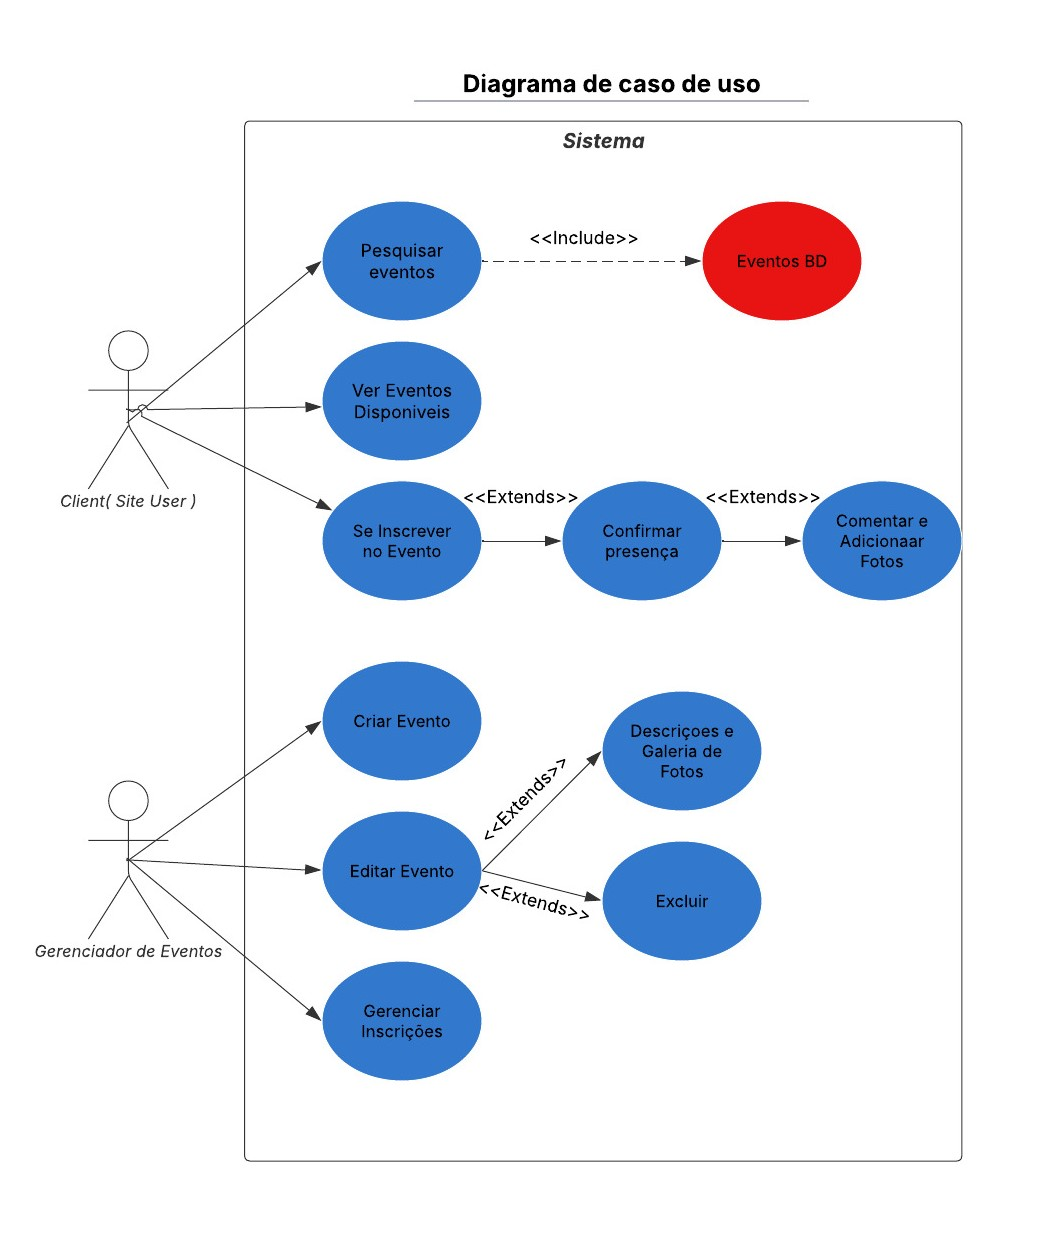
\includegraphics[width=0.6\textwidth]{images/user_case}
  \caption{Diagrama de Casos de Usos}
  \label{fig:diagram_user_case}
\end{figure}

\section{Diagrama ER}
\textit{CriasEvent} irá tratar uma entidade usuario que pode vir a ter 3 cargos:
\begin{itemize}
    \item Cliente
    \item Organizador
    \item Administrador
\end{itemize}
\textit{CriasEvent} com base no "Ranking" deste usuario ele terá acesso a funcionalidades espeficicas de edição geral. \par
A imagem a seguir demonstra um Diagrama de Entidade Relacionamento, para um entendimento base dos relacionamentos entre as atividades fornecidas ao Usuario.
\begin{figure}[h]
  \centering
  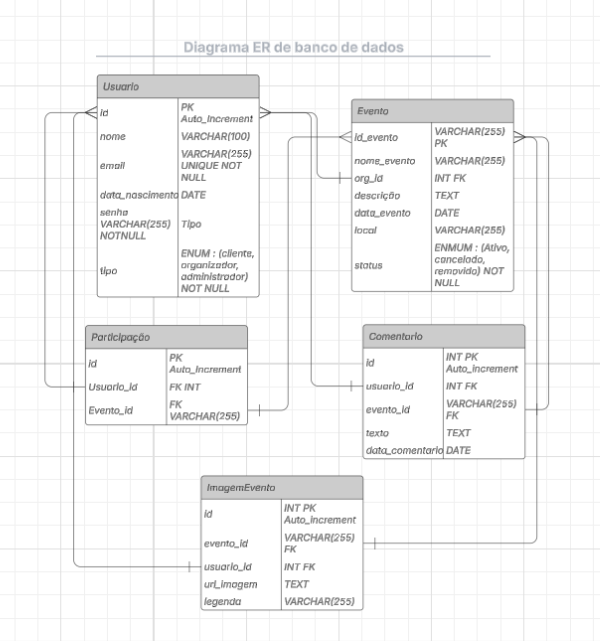
\includegraphics[width=0.8\textwidth]{images/diagrama_ER.png}
  \caption{Diagrama de Entidade Relacionamento}
  \label{fig:diagram_Entity_Relatioship}
\end{figure}

\section{Tabela Usuario}
A tabela usuario é fundamental para o estabelecimento das pessoas as quais usaram o \textit{CriasEvent}. Há 3 possibilidades distintas de usuarios sendo estes os previamente dito:
\begin{itemize}
    \item Cliente
    \item Organizador
    \item Administrador
\end{itemize}
Cliente é o usuario padrao do site, ao qual consumira os eventos gratuitos, Organizador de eventos será responsavel por criar o evento, edita-lo e monitorar seu acontecimento e o Administrador do site ficará responsavel por manter a ordem no site, tendo todas permissoes.
Comentarios breves a respeito de suas variaveis:
\begin{itemize}
    \item Id : Chave primaria para indentificar o Usuario, sendo esta chave UNICA.
    \item nome : Nome do usuario.
    \item email : Email do Usuario.
    \item dataNascimento : Data de nascimento do usuario.
    \item senha : senha do Usuario
    \item tipo : Previamente mencionado, os tipos de usuario possiveis (Cliente, Organizador ou Administrador).
\end{itemize}

\section{Tabela Evento}
\textit{CriasEvent} fornece a possibilidade para o usuario Cliente se inscrever a um evento, para tal atividade sera necessario informacoes fundamentais no processo de criacao do evento aos quais sao armazenados na tabela Evento.

\begin{itemize}
    \item idEvento : Chave primaria para indentificacao do evento.
    \item nomeEvento : Nome inserido pelo organizador do evento.
    \item orgId : Chave estrangeira para identificacao do Organizador de eventos, utilizando seu Id armazenado.
    \item descricao : Organizador de evento pode descrever o evento nesta área.
    \item dataEvento : Data quando ocorrera o evento.
    \item local : Local onde ocorrera o evento.
    \item status : 3 Possibilidades distintas em que se pode encontrar o evento, sendo Ativo, Cancelado ou Removido.
\end{itemize}

\section{Tabela Participacao}
Tabela com foco em armazenar os Clientes e os eventos aos quais estes participam.
\begin{itemize}
    \item Id : chave para propria participacao.
    \item UsuarioId : Anexa o Id do usuario para agrupamento de usuario e evento.
    \item EventoId : Anexa o Id do usuario para agrupamento de evento e usuario.
\end{itemize}

\section{Comentario}
Tabela para obter os comentarios relacionados ao evento em questao, além de anexa-los ao usuarios que os fizeram.

\begin{itemize}
    \item Id : Chave primaria de cada comentario realizado.
    \item UsuarioId : Chave estrangeira para identificacao de usuario que comentou no evento
    \item eventoId : Chave estrangeira para identificacao do evento ao qual foi realizado o comentario sobre.
    \item texto : Comentario realizado.
    \item dataComentario : Data qual comentario foi realizado.
\end{itemize}

\section{ImagemEvento}
Imagem aderida ao evento, esta inclusao é feita tanto pelo usuario, para postar sobre o evento ocorrido, ou até mesmo para promover o evento pelo organizador.

\begin{itemize}
    \item id : chave primaria para identificacao da imagem.
    \item eventoId : chave estrangeira para identificacao do evento.
    \item usuarioId : chave estrangeira para identificao do usuario ao qual realizou a postagem.
    \item urlImagem : Endereco da imagem postada.
    \item legenda : Breve descricao para imagem postada.
\end{itemize}

\section{Explicacao dos Relacionamentos}
\begin{tabular}{>{\raggedright}p{1.5cm}>{\raggedright}p{4cm}>{\raggedright}p{4cm}>{\raggedright}p{6cm}}
\toprule
  \textbf{ID} & \textbf{Relacionamento FK} &\textbf{Relacionamento PK} & \textbf{Descrição}  \tabularnewline 
\midrule
  1 & Participacao(usuarioId) & Usuario(id) & Obtencao do id na tabela de usuario para marcar sua presenca no evento. 
  \tabularnewline \hline
  2 & Participacao(EventoId) & Evento(idEvento) & Variavel importante para anexar a presenca do usuario ao evento respectivo da sua participacao
  \tabularnewline \hline
  3 & Evento(orgId) & Usuario(Id) & Para criacao do evento precisa-se de um Organizador de eventos para tal ato, id deste Organizador armazenado. \tabularnewline \hline
  4 & Comentario(usuarioId)& Usuario(Id) & Vincula o comentario armazenado ao Usuario que o fez. 
  \tabularnewline \hline
  5 & Comentario(eventoId) & Evento(idEvento) & Comentario sera anexado na pagina a um evento respectivo, para isso vincula-o ao EventoId. \tabularnewline \hline
  6 & ImagemEvento(usuarioId) & Usuario(Id) & Para postagem da foto, vincula o usuario a imagem por meio do Id. 
  \tabularnewline \hline
  7 & ImagemEvento(EventoId) & Evento(EventoId) & Anexa a imagem ao evento com auxilio do ID de evento.
  \tabularnewline \hline
\bottomrule
\end{tabular}


\chapter{Requisitos}
\label{Requisitos}

\section{Requisitos Funcionais Página Web}

\begin{tabular}{>{\raggedright}p{1.5cm}>{\raggedright}p{4cm}>{\raggedright}p{10cm}}
\toprule
\textbf{ID} & \textbf{Requirement} & \textbf{Description} \tabularnewline 
\midrule
  RF101 & Homepage & Pagina inicial exibindo os eventos disponiveis, caixa de busca e botão de cadastro.\tabularnewline \hline
  RF102 & Cadastro/Login & Pagina de Cadastro com caixas de informações para preenchimento e possibilidade de login direto.\tabularnewline \hline
  RF103 & Gerenciamento de Evento (Organizador) & Pagina exclusiva para Usuário Organizador onde será possível realizar o Crud dos eventos\tabularnewline \hline 
  RF104 & Busca de Eventos & Realizar a busca e filtragem de eventos da Homepage baseado em palavras-chave.\tabularnewline \hline
  RF105 & Inscrição Eventos & Página para inscrição no evento selecionado.\tabularnewline \hline
  RF106 & Página de Usuário & Página com as informçãoes do usuário, e.g.: Eventos incritos/gerenciados e informações de cadastro.\tabularnewline \hline
  RF107 & Página de Evento & Página com a informação do evento selecionado.\tabularnewline
\bottomrule
\end{tabular}

\section{Requisitos Funcionais Banco de Dados}
\begin{tabular}{>{\raggedright}p{1.5cm}>{\raggedright}p{4cm}>{\raggedright}p{10cm}}
\toprule
\textbf{ID} & \textbf{Requirement} & \textbf{Description} \tabularnewline 
\midrule
  RF201 & Criação de evento & Permitir ao usuário criar um evento, atribuindo as informações necessárias.\tabularnewline \hline
  RF202 & Consulta de evento & Filtrar eventos com base em informações e palavras chaves\tabularnewline \hline
  RF203 & Atualizção de evento & Adicionar, remover ou alterar informções sobre o evento.\tabularnewline \hline
  RF204 & Remoção de evento & Excluir um evento.\tabularnewline \hline
  RF205 & Gerar Lista de Presença & Exportar uma lista de inscritos no evento.\tabularnewline 
\bottomrule
\end{tabular}

\section{Requisitos Funcionais Backend}

\begin{tabular}{>{\raggedright}p{1.5cm}>{\raggedright}p{4cm}>{\raggedright}p{10cm}}
\toprule
\textbf{ID} & \textbf{Requirement} & \textbf{Description} \tabularnewline 
\midrule
  RF301 & Pedidos de Leitura & Comunicar pedidos de leitura de informção do Banco de dados feitos pela webpage. \tabularnewline \hline
  RF302 & Pedidos de Escrita & Comunicar pedidos de Escrita de informações no Banco de dados feitos pela webpage.\tabularnewline \hline
  RF303 & Pedidos de Remoção & Comunicar pedidos de remoção de informações ou de eventos em si do banco de dados feitos pela webpage.\tabularnewline \hline
  RF304 & Pedidos de Atualização & Comunicar pedidos de atualização de informção, tanto de usuários quanto de eventos, feitos pela web page ao banco de dados.\tabularnewline 
\bottomrule
\end{tabular}


\section{Requisitos não funcionais}
\begin{tabular}{>{\raggedright}p{1.5cm}>{\raggedright}p{4cm}>{\raggedright}p{10cm}}
\toprule
\textbf{ID} & \textbf{Requirement} & \textbf{Description} \tabularnewline 
\midrule
RNF001 & Sistema de notificações & Organizadores poderão se comunicar com os inscritos por e-mail ou mensagens no sistema, participantes receberão notificações sobre novos eventos, alterações em eventos inscritos etc. \tabularnewline \hline
RNF002 & Perfis para organizadores e participantes. & Os perfis devem mostrar informações sobre seu usuário, como Histórico de eventos participados e/ou organizados. \tabularnewline \hline
RNF003 & Sistema de Upload multimidia & Permitir que os usuários postem fotos e vídeos. \tabularnewline \hline 
RNF-008 & Sistema de comentarios & Permitir comentarios em fotos.\tabularnewline

\bottomrule
\end{tabular}


\chapter{Restrições e Riscos}

\section{Restrições}
    O sucesso do projeto pode ser interrompido se um ou mais do seguintes fatores ocorrerem:
    \begin{itemize}
        \item Falha de atender aos requerimentos listados pela entidade superior.
        \item Falha de se cumprir com o prazo de entrega determindado.
        \item Incapacidade dos autores de implementarem as funcionalidades exigidas por conta de falta de conhecimento da utilização das ferramentas necessárias.
    \end{itemize}


\section{Definição de Risco}

\begin{appendices}
\chapter{Glossário}
\begin{itemize}
 \item CriasEvent: Nome do sistema de gerenciamento de eventos que está sendo desenvolvido. O objetivo principal é permitir que organizadores criem e gerenciem eventos e que participantes possam se inscrever neles

\item Organizadores: Classe de usuários do CriasEvent que têm a capacidade de criar e gerenciar eventos na plataforma Eles podem executar operações de CRUD (criar, ler, atualizar e excluir) nos dados dos eventos.

\item Participantes: Classe de usuários do CriasEvent que podem buscar e se inscrever nos eventos disponíveis.

\item Administrador: Classe de usuários do CriasEvent que têm controle sobre todo o conteúdo do site.

\item Evento: Uma ocorrência, tanto presencial quanto online, que pode ser criada e gerenciada por organizadores através do sistema CriasEvent. O sistema permite o preenchimento de informações, upload de imagens e definição de vagas para eventos.

\item Inscrição: O processo pelo qual os participantes demonstram interesse em participar de um evento através do sistema CriasEvent . O sistema também oferece gerenciamento de inscrições, incluindo confirmação e lista de presença 

\item CRUD: Acrônimo para as operações fundamentais de Criar, Read (Ler), Update (Atualizar) e Delete (Excluir) dados no banco de dados. No contexto do CriasEvent, os organizadores utilizarão essas operações para gerenciar os eventos . O banco de dados para essas operações será o MySQL.

\item Requisitos Funcionais: Descrevem as funcionalidades que o sistema CriasEvent deverá implementar, ou seja, o que o sistema deverá ser capaz de fazer. Exemplos incluem o CRUD de eventos, a criação da página web, a busca e filtro de eventos e o gerenciamento de inscrições.

\item Requisitos Não Funcionais: Descrevem as qualidades ou restrições do sistema CriasEvent, como desempenho, usabilidade, segurança, etc. Exemplos incluem o sistema de notificações, perfis para organizadores e participantes e a integração com redes sociais.
\end{itemize}
\end{appendices}


